\chapter{Variedades Complejas}

\section{Definición}

La categoría protagonista de todo el trabajo es la categoría de las \textit{variedades compleja}. Los objetos que estudiaremos serán espacios Hausdorff que se modelan localmente como abiertos de $\cc^n$ y esto permite extender los conceptos del análisis complejo clásico a un contexto de geometría global.

\begin{definition}
        Sea $M$ un espacio topológico Hausdorff y segundo numerable. Decimos que $M$ es una \textbf{variedad compleja} (de dimensión $n$) si existe un par $\{(U_i,\varphi_i)\}$ tales que
        \begin{enumerate}
            \item $\{U_i\}_{i\in I}$ es una cubierta abierta de $M$.
            \item Para cada $i\in I$, se tiene que $\varphi_i:U_i\to\varphi_i(U_i)\subset \cc^n$ es un homeomorfismo.
            \item Para cada $i,j\in I$, si $U_i\cap U_j\neq\emptyset$ entonces la aplicación
            \begin{equation*}
                \varphi_{ij}=\varphi_j\circ\varphi_i^{-1}:\varphi_i(U_i\cap U_j)\to\varphi_j(U_i\cap U_j),
            \end{equation*}
            llamada \textbf{función de transición}, es holomorfa.
            \begin{figure}[H]
            	\centering
            	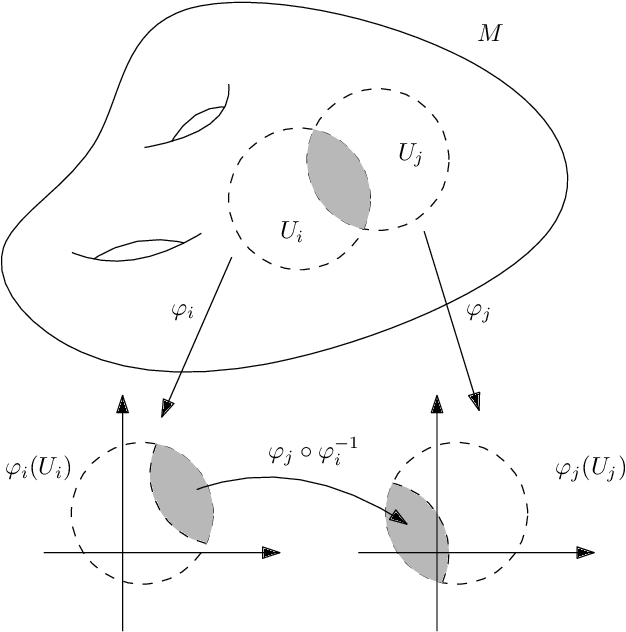
\includegraphics[width=0.3\linewidth]{Imagenes/atlas holomorfo}
            	\caption{Representación de cartas holomorfa.}
            	\label{fig:atlas-holomorfo}
            \end{figure}
            
        \end{enumerate}
        El par $(U_i,\varphi_i)$ es llamado \textbf{carta holomorfa} y la colección $\{(U_i,\varphi_i)\}$ de todas las cartas es llamado \textbf{atlas holomorfo}. Si existe un atlas holomorfo para $M$, también vamos a decir que \textbf{admite una estructura analítica}.
        Una \textbf{curva compleja} es una variedad compleja de dimensión $1$, y si además es conexa le llamamos \textbf{superficie de Riemann}. Por último, decimos que una variedad compleja de dimensión $2$ es una \textbf{superficie compleja}.
    \end{definition}

    Ahora vamos a presentar varios ejemplos esenciales de variedades complejas.
    
    \begin{example}[$ n $-espacio afín $\cc^n$]   
        Consideremos el espacio complejo $\cc^n$. Un atlas holomorfo para este espacio está dado por $\mathscr{A}=\{(\cc^n,\mathrm{id})\}$\footnote{Note que no es un atlas maximal.}, además de cumplir con todas las propiedades topológicas que necesitamos para ser una variedad compleja. Este será nuestro ejemplo base de variedad compleja no compacta. 
    \end{example}
    
    \begin{example}[Abierto de una variedad]
    	Si $M$ es una variedad compleja con atlas holomorfo $\{(U_i,\varphi_i)\}$, entonces todo abierto no vacío $U\subset M$ es una variedad compleja con atlas holomorfo $\{(U\cap U_i,\varphi_i|_{U\cap U_i})\}$.
    \end{example}

	\begin{example}[Producto de variedades]
		Si $M_1,\dots, M_k$ son variedades complejas de dimensión $n_1,\dots,n_k$ respectivamente. Entonces el producto $M_1\times \cdots\times M_k$ es una variedad compleja de dimensión $n_1+\cdots+n_k$ cuyas cartas son de la forma $(U_1\times\cdots\times U_k,\varphi_1\times\cdots\times \varphi_k)$. Notemos que las cartas son compatibles pues
		\begin{equation*}
			(\psi_1\times\cdots\times \psi_k)\circ (\varphi_1\times\cdots\times \varphi_k)^{-1}=(\psi_1\circ\varphi_1^{-1})\times\cdots\times (\psi_k\circ \varphi_k^{-1})
		\end{equation*}
		es una aplicación holomorfa.
	\end{example}
	
    \begin{example}[Toro Complejo]
        Consideremos $V$ un $\cc$-espacio vectorial de dimensión $n$. Una \textbf{retícula} en $V$ es un subgrupo aditivo abeliano discreto $\Lambda\subset V$ generada por $2n$ vectores $v_1,\cdots,v_{2n}$ los cuales son linealmente independientes sobre $\rr$. El cociente $V/\Lambda$ es una variedad compleja de dimensión $n$ compacta y conexa (véase \parencite[Example 1.18]{leecomplex}). Además, se puede determinar un difeomorfismo entre $V/\Lambda$ y el producto de círculos $(S^1)^{2n}$.
        Un caso particularmente interesante es el cociente 
        \begin{equation*}
            T=\cc/\Lambda
        \end{equation*}
        donde $\Lambda=w_1\zz+w_2\zz$ y $w_1,w_2$ son linealmente independientes sobre $\rr$. Esta curva compleja es llamada \textbf{curva elíptica}.
		\begin{figure}[H]
			\centering
			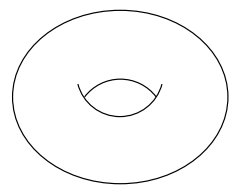
\includegraphics[width=0.25\linewidth]{Imagenes/toro}
			\caption{Modelo topológico de las curvas elípticas.}
			\label{fig:toro}
		\end{figure}
    \end{example}
    
%    \begin{example}[Variedades de Hopf]
%    	Consideremos $\lambda=(\lambda_1,\dots,\lambda_n)$ una $n$-tupla ordenada de números reales tal que $0<\lambda_i<1$, y definamos la acción $\cdot:\zz\times\cc^n\setminus\{0\}\to\cc^n\setminus\{0\}$ dada por
%    	\begin{equation*}
%    		k\cdot z=((\lambda_1)^kz_1,\dots,(\lambda_n)^kz_n).
%    	\end{equation*}
%    	Esta acción es holomorfa, libre y propia, por lo que el cociente bajo esta acción
%    	\begin{equation*}
%    		H=\frac{\cc^n\setminus\{0\}}{\zz}
%    	\end{equation*}
%    	es una variedad compleja conexa y compacta llamada \textbf{variedad de Hopf}. Más aún, esta variedad $H$ es difeomorfa a $S^{2n-1}\times S^1$. (veáse \parencite[Example 1.19]{leecomplex})
%    \end{example}
    
    Ahora vamos a ver con detalle cómo los ceros de funciones holomorfas determinan variedades complejas. Lo anterior es fundamental para determinar la estructura analítica de las variedades algebraicas, pues los polinomios son funciones holomorfas.
    
    \begin{example}[Hipersuperficie afín]
        Consideremos una función holomorfa $f:\cc^n\to \cc$ con $0\in\cc$ un valor regular. Sea
        \begin{equation*}
            X:=f^{-1}(0)=Z(f)\subset \cc^n
        \end{equation*}
        y $p\in X$. Escribiendo $f=f(z_1,\dots,z_n)$, el jacobiano de $f$ en $p$ está dado por
        \begin{equation*}
        	J(f)(p)=\left(\frac{\partial f}{\partial z_1}(p),\dots, \frac{\partial f}{\partial z_n}(p)\right).
        \end{equation*}
  		Como $0\in\cc$ es un valor regular, entonces $p$ es un punto regular. Así, el rango de la matriz $J(f)(p)$ (de tamaño $1\times n$) es $1$, es decir, al menos una derivada parcial no se anula en $p$. Sin pérdida de generalidad, podemos asumir que 
  		\begin{equation*}
  			\frac{\partial f}{\partial z_n}(p)\neq 0.
  		\end{equation*}
        En particular, existe una vecindad $U\subset\cc^n$ de $p$ donde $\frac{\partial f}{\partial z_n}$ no se anula. Renombrando las coordenadas $w=(z_1,\dots,z_{n-1})$ y $z=z_n$, se puede escribir $f=f(w,z)$. Por el teorema de la función implícita \ref{funcionimplicita}, existe una vecindad $W\subset\cc^{n-1}$ de $w_0=(p_1,\dots,p_{n-1})$ y una función holomorfa $g:W\to\cc$ tal que $f(w,g(w))=0$ para todo $w\in W$ y  
        \begin{equation*}
        	\{(w,z)\in W\times\cc:f(w,z)=0\}=\{(w,g(w)):w\in W\}.
        \end{equation*}
    	Definamos ahora la función
    	\begin{align*}
    		\varphi:X\cap U&\longrightarrow W\subset\cc^{n-1}\\
    		(w,z)&\longmapsto w.
    	\end{align*}
    	\begin{center}
    		\begin{figure}[H]
    			\centering
    			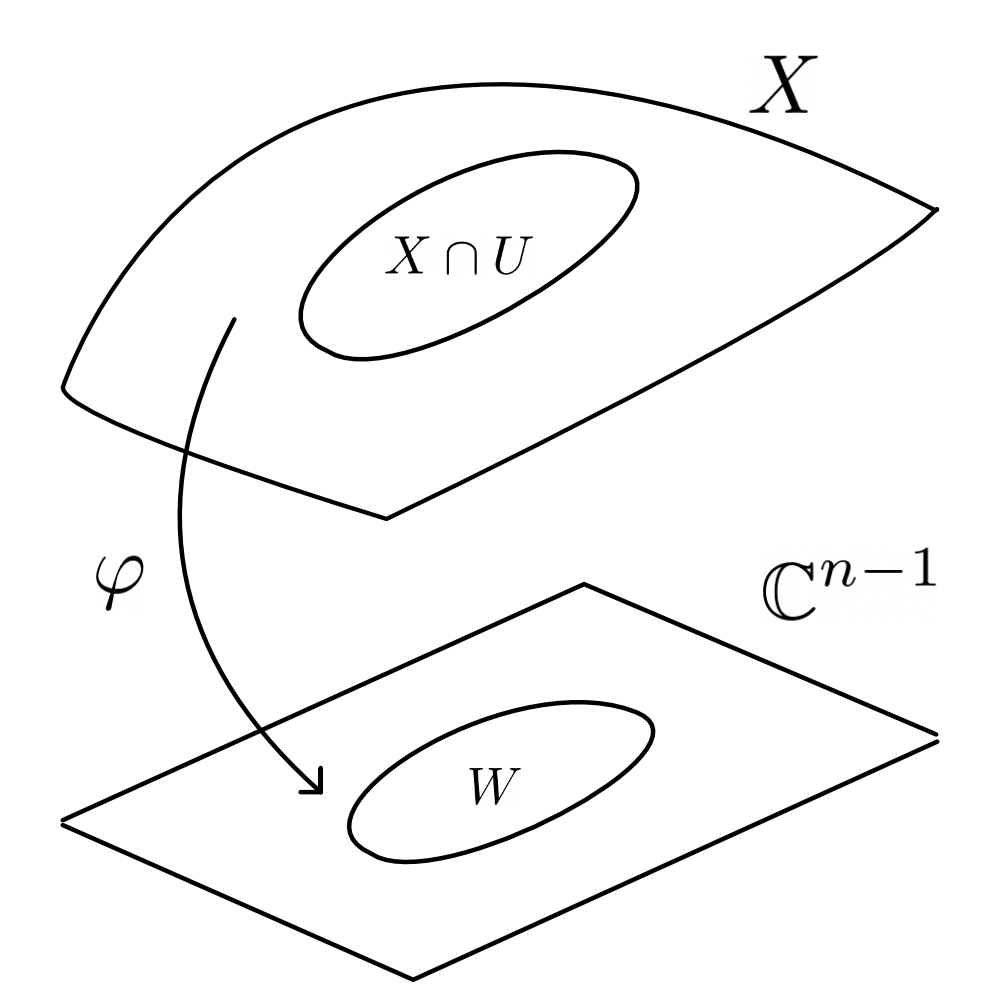
\includegraphics[width=0.3\linewidth]{Imagenes/hipersuperficie afin}
    			\caption{Carta de la hipersuperficie afín.}
    			\label{fig:hipersuperficie-afin}
    		\end{figure}
    	\end{center}
    	Queremos ver que $\varphi$ es una carta para $p$. Probemos primero que es inyectiva y sobreyectiva.
    	\begin{itemize}
    		\item Sean $x,x'\in X\cap U$ tales que $\varphi(x)=\varphi(x')$. Si $x=(w,z)$ y $x'=(w',z')$, entonces $z=g(w)$ y $z'=g(w')$. Así,
    		\begin{align*}
    			\varphi(x)&=\varphi(x')\\
    			w&=w'
    		\end{align*}
    		De esta forma, $z=z'$ y por tanto $x=x'$. Esto significa que $\varphi$ es inyectiva.
    		\item Sea $w\in W$, entonces $(w,g(w))\in X\cap U$ y
    		\begin{equation*}
    			\varphi(w,g(w))=w.
    		\end{equation*}
    		Así, $\varphi$ es sobreyectiva.
    	\end{itemize}
    	Con esto, $\varphi$ es biyectiva y además la inversa de $\varphi$ está dada por
    	\begin{align*}
    		\varphi^{-1}:W\to X\cap U\\
    		w\mapsto (w,g(w))
    	\end{align*}
 
    	Como $\varphi$ y $\varphi^{-1}$ son aplicaciones holomorfas, en particular son funciones continuas.
    	Dado que todo punto de $X$ es regular, para cada $p\in X$ existe un abierto $U$ y una carta centrada en $p$. Ahora probemos que las funciones de transición son holomorfas.\\
    	Sea $p\in X\cap U$ otro punto con carta $\psi:X\cap U'\to W'$, entonces
    	\begin{equation*}
    		\psi\circ\varphi^{-1}:\varphi((X\cap U)\cap(X\cap U'))\to\psi((X\cap U)\cap(X\cap U'))
    	\end{equation*}
    	es una función tal que 
    	\begin{equation*}
    		w\mapsto (w',g(w'))\mapsto w'
    	\end{equation*}
    	donde $w'$ es la proyección sobre las $n-1$ coordenadas elegidas por la carta $\psi$. Dado que ambas proyecciones son holomorfas, entonces la función de transición $\psi\circ\varphi^{-1}$ es holomorfa. Como $\varphi^{-1}$ está dada por $(w,g(w))$ y $\psi$ es una proyección de coordenadas, la composición $\psi\circ\varphi^{-1}$ es holomorfa.
    	De esta manera, las cartas $(X\cap U,\varphi)$ dotan a $X$ de un atlas holomorfo.\\
    	Más aún, $X$ como subespacio de $\cc^n$ es un espacio Hausdorff, segundo numerable y con estructura holomorfa. Por lo tanto, $X$ es una variedad compleja de dimensión $n-1$.
    \end{example}

    Generalizando este último ejemplo tenemos:
    \begin{example}[Intersección compleja]\label{interseccioncompleja}
        Sean $k$ funciones holomorfas $f_1,f_2,\cdots,f_k:\cc^n\to \cc$, con $k\leq n$ y definamos la aplicación holomorfa asociada
        \begin{equation*}
        	f=(f_1,\dots,f_k):\cc^n\to\cc^k.
        \end{equation*}   
    	Supongamos que $0\in\cc^k$ es un valor regular de $f$. Entonces el conjunto
    	\begin{equation*}
    		X:=f^{-1}(0)=Z(f_1)\cap\cdots\cap Z(f_k)=Z(f_1,\dots,f_k)
    	\end{equation*}
    	es una variedad compleja de dimensión $n-k$.\\
    	La demostración sigue la misma estrategia para el caso $k=1$ con ciertas observaciones:
    	\begin{itemize}
    		\item Para cada punto $p\in X$, el rango de la matriz jacobiana $J(f)(p)$ es $k$. Por una renumeración de las variables, podemos suponer que la submatriz cuadrada de las últimas $k$ variables tiene determinante no cero.
    		\item Por el teorema de la función implícita, tenemos una vecindad $W\subset\cc^{n-k}$ de las primeras $n-k$ entradas de $p$, una vecindad $Z\subset\cc^k$ de las últimas $k$ entradas de $p$ y una aplicación holomorfa
    		\begin{equation*}
    			g:W\to Z
    		\end{equation*}
    		\item Las cartas $\varphi:X\cap U\to W\subset\cc^{n-k}$ se construyen de la misma manera y la transición sigue siendo holomorfa como antes, por componerse de proyecciones y las funciones holomorfas $g$.
    	\end{itemize}
    	
    \end{example}

	\begin{example}[Espacio proyectivo]
		El \textbf{n-espacio proyectivo} es el conjunto $\pp^n=\cc^{n+1}\setminus\{0\}/\sim$ donde $z,w\in\cc^{n+1}\setminus\{0\}$ están relacionados si, y solo si, existe $\lambda\in\cc\setminus\{0\}$ tal que  $z=\lambda w$.
		
		Dotamos a $\pp^n$ con la topología cociente dada por la proyección canónica
		\begin{equation*}
			q:\cc^{n+1}\setminus \{0\} \longrightarrow \pp^n
		\end{equation*}
		Consideremos la cubierta estándar afín de $\pp^n$ dada por los $n+1$ abiertos
		\begin{equation*}
			U_i=\{[x_0:\cdots:x_n]:x_i\neq 0\}\subset \pp^n
		\end{equation*}
		Así, tenemos las funciones $\varphi_i:U_i\to\cc^n$ dadas por
		\begin{align*}
			[x_0:x_1:\dots:x_n]\mapsto & \left( \frac{x_0}{x_i},\frac{x_1}{x_i},\dots, \frac{x_{i-1}}{x_i},\frac{x_{i+1}}{x_i},\dots,\frac{x_n}{x_i}\right)
		\end{align*} 
		Estas funciones son continuas por la propiedad característica de la topología cociente y su inversa está dada por
		\begin{equation*}
			\varphi_{i}^{-1}(z_1,\dots,z_n)=[z_1:\dots:z_{i-1}:1:z_{i+1}:\dots:z_n]
		\end{equation*}
		Así, las funciones $\varphi_i$ son homeomorfismos llamados \textbf{cartas afines}.
		Además, las funciones de transición $\varphi_{ij}=\varphi_i\circ\varphi_j^{-1}:\varphi_j(U_i\cap U_j)\to\varphi_i(U_i\cap U_j)$ están dadas por
		\begin{equation*}
			\varphi_{ij}(w_1,\dots,w_n)=\left(\frac{w_1}{w_i},\dots \frac{w_{i-1}}{w_i},\frac{w_{i+1}}{w_i},\dots,\frac{w_{j-1}}{w_i},\frac{1}{w_i},\frac{w_{j+1}}{w_i},\dots,\frac{w_n}{w_i} \right)
		\end{equation*}
		Notemos que $\varphi_i(U_i \cap U_j)=\cc^n\setminus Z(w_j)$. Con esto, las funciones $\varphi_{ij}$ son aplicaciones holomorfas.\\
		Las propiedades topológicas de Hausdorff y segundo numerable son análogas al caso de $\pp^1$ (véase \parencite[Cap. 1, Sec. 1, Ejem. 1.3]{zaldrimann}).\\
		Si consideramos la esfera $S^{2n+1}$ unitaria de $\cc^{n+1}$, entonces tenemos la siguiente composición de funciones continuas\footnote{A la tríada $(S^{2n+1},q,\pp^n)$ se le llama \textbf{fibrado de Hopf}.}
		\[\begin{tikzcd}
			{S^{2n+1}} && {\cc^{n+1}\setminus\{0\}} \\
			\\
			&& {\mathbb{P}^n}
			\arrow[hook, from=1-1, to=1-3]
			\arrow["\rho"', dashed, from=1-1, to=3-3]
			\arrow["p", two heads, from=1-3, to=3-3]
		\end{tikzcd}\]
		Como $\pp^n$ es la imagen continua de $S^{2n+1}$ bajo $\rho$ y la esfera es conexa y compacta, entonces podemos concluir que el espacio proyectivo $\pp^n$ es conexo y compacto.
		Por lo tanto, $\pp^n$ es una variedad compleja conexa y compacta.
	\end{example}
	\begin{figure}[H]
		\centering
		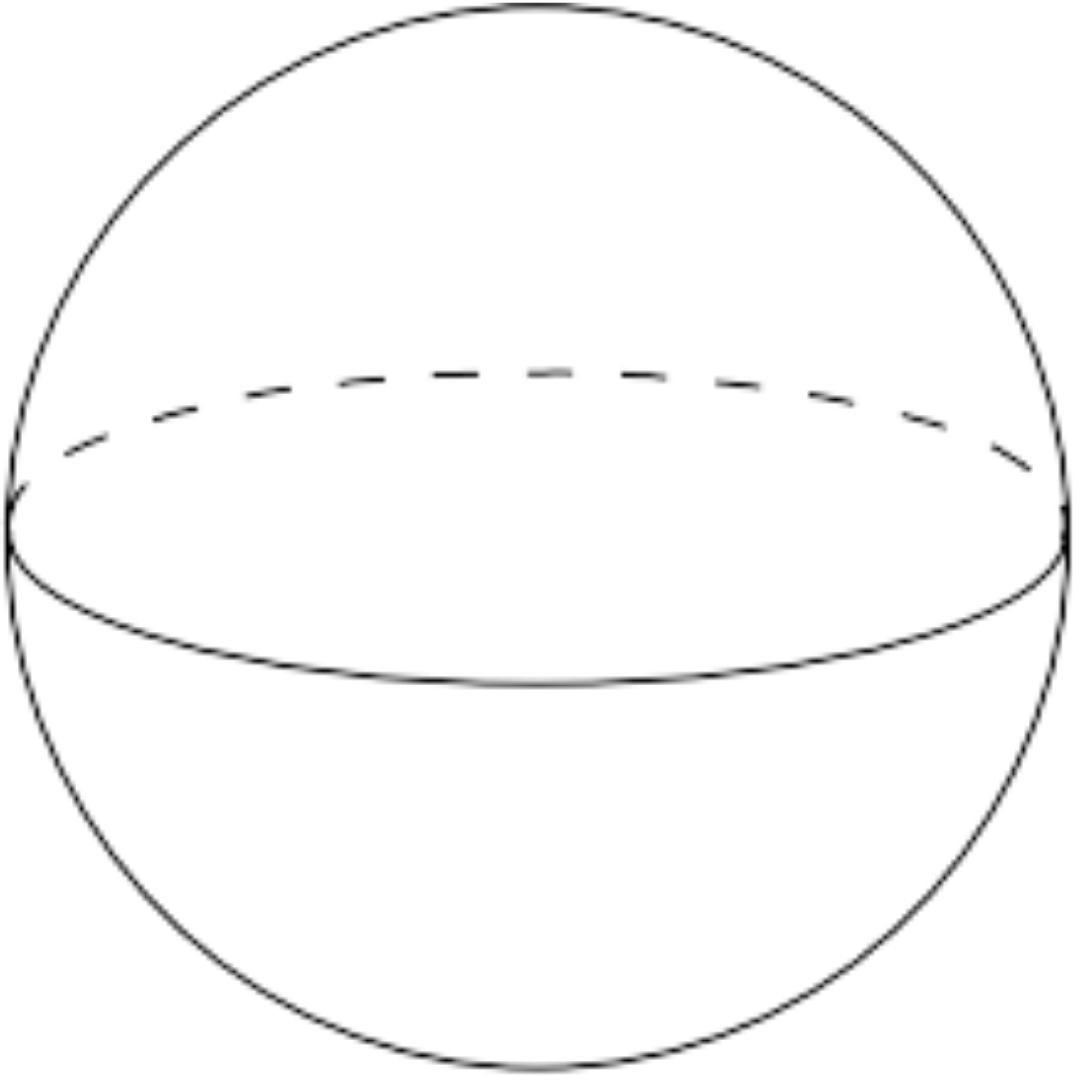
\includegraphics[width=0.2\linewidth]{Imagenes/Esfera}
		\caption{Recta proyectica $\pp^1$}
		\label{fig:esfera}
	\end{figure}
	
	
    En este trabajo nos enfocaremos principalmente en las variedades compactas conexas, pues muchos resultados importantes se sustentan bajo estas hipótesis y son esenciales para el tema de algebrización. Veremos con más detalle esto último en el tercer capítulo.
    
\section{Aplicaciones Holomorfas}
	
	Pese a que las funciones holomorfas son suaves, estas mismas tienen una rigidez mucho mayor que las funciones suaves en la geometría diferencial real. Como en el análisis complejo, esta diferencia tiene consecuencias profundas en el estudio de estos objetos, y en consecuencia también cambia la situación geométrica con respecto a la real. Por ejemplo, en la geometría diferencial real la orientabilidad es una condición adicional y fundamental para teoremas importantes, en geometría compleja se demuestra que toda variedad compleja es orientable. Por otra parte, la estructura del anillo de funciones holomorfas globales sobre una variedad compleja compacta es altamente restrictiva (véase teorema \ref{holomorfasglobal}).
	
	Vamos a establecer las formalidades sobre morfismos entre variedades complejas en fin de comprender la riqueza analítica de las mismas.
    
    \begin{definition}[Aplicación holomorfa]
        Sean $M$ y $N$ dos variedades complejas. Una \textbf{aplicación holomorfa} entre $M$ y $N$ es una función continua $f:M\to N$ tal que para cada $p\in M$, para cada carta $(U,\varphi)$ alrededor de $p\in M$ y $(V,\psi)$ alrededor de $f(p)\in N$, la función
        \begin{equation*}
            \psi\circ f\circ \varphi^{-1}:\varphi(U\cap f^{-1}(V))\longrightarrow\psi(V)
        \end{equation*}
        es una aplicación holomorfa en $\varphi(p)$.
        \begin{center}
            \begin{tikzcd}
			{p\in U} && {f(p)\in V} \\
			\\
			{\varphi(U\cap f^{-1}(V))} && {\psi(V)}
			\arrow["f", from=1-1, to=1-3]
			\arrow["\varphi"', from=1-1, to=3-1]
			\arrow["\psi", from=1-3, to=3-3]
			\arrow["{\psi\circ f\circ \varphi^{-1}}"', from=3-1, to=3-3]
		\end{tikzcd}
        \end{center}
    \end{definition}

    \begin{definition}
        Una aplicación holomorfa $f:M\to N$ entre variedades complejas se llama \textbf{biholomorfismo} si es biyectiva y su inversa también es una aplicación holomorfa. Dos variedades complejas se dicen \textbf{biholomorfas} si existe un biholomorfismo entre ellas.
    \end{definition}

    \begin{remark}
        Dada una función continua $f:M\to N$, la propiedad de ser holomorfa es independiente de la elección de las cartas holomorfas de la estructura holomorfa de $M$ y $N$. Así, la verificación de la propiedad puede realizarse para cualquier atlas de $M$ y $N$.
    \end{remark}

    \begin{lemma}$ $
        \begin{enumerate}
            \item La restricción de una aplicación holomorfa a un subconjunto abierto es holomorfa.
            \item Toda aplicación constante entre variedades complejas es una aplicación holomorfa.
            \item La aplicación identidad sobre cualquier variedad compleja es una aplicación holomorfa.
            \item Toda carta holomorfa es un biholomorfismo sobre su imagen.
            \item La composición de aplicaciones holomorfas es una aplicación holomorfa.
        \end{enumerate}
    \end{lemma}

    Tenemos muchos resultados enigmáticos de las funciones holomorfas y resulta interesante ver sus consecuencias en las aplicaciones holomorfas entre variedades complejas. Uno de los más importantes, y una primera distinción frente a las variedades reales, es el \textit{teorema de la identidad}.

    \begin{theorem}[Teorema de la identidad]\label{teoidentidad}
        Sean $M$ y $N$ dos variedades complejas, con $M$ conexa y $f,g:M\to N$ dos aplicaciones holomorfas que coinciden en un subconjunto abierto no vacío de $M$. Entonces $f=g$. 
    \end{theorem}
	\begin{proof}
		Comencemos definiendo el conjunto
		\begin{equation*}
			A=\{p\in M:f\text{ y }g\text{ coinciden en una vecindad de }p\ \}.
		\end{equation*}
		Queremos demostrar que este conjunto es abierto y cerrado. Dado que $M$ es conexo, tendríamos que $A=M$.
		\begin{itemize}
			\item Sea $p\in A$, entonces existen cartas $(U,z)$ alrededor de $p$ y $(V,w)$ en $N$ tales que
			\begin{equation*}
				f(U),g(U)\subset V.
			\end{equation*}
			Como $f$ y $g$ son aplicaciones holomorfas, entonces las funciones $w\circ f\circ z^{-1}$ y $w\circ g\circ z^{-1}$ son holomorfas en $z(U)$. Además, como $p\in A$ entonces existe una vecindad $W\subset M$ de $p$ donde $f$ y $g$ coinciden. Así,
			\begin{equation*}
				(w\circ f\circ z^{-1})\left.\right|_{z(U\cap W)}=(w\circ g\circ z^{-1})\left.\right|_{z(U\cap W)}.
			\end{equation*} 
			Por el teorema de la identidad \ref{identidad}, las funciones coinciden en todo $z(U)$.
			Por lo que, $f=g$ en todo $U$ y $U\subset A$.\\
			De esta forma, $p$ es un punto interior de $A$ y concluimos que $A$ es un conjunto abierto.
			
			\item Supongamos que $b\in \partial A$. Queremos probar que $b\in A$ para concluir que $A$ es cerrado.
			Como $b$ pertenece a la frontera de $A$ y $f$ y $g$ coinciden en $A$, por continuidad tenemos que $f(b)=g(b)$. Tomemos cartas $(U,z)$ de $M$ alrededor de $b$ y $(V,w)$ de $N$ alrededor de $f(b)=g(b)\in N$, con $U$ conexo. Definamos
			\begin{align*}
				F&=w\circ f\circ z^{-1}:z(U)\to w(V),\\
				G&=w\circ g\circ z^{-1}:z(U)\to w(V),
			\end{align*}
			las cuales son holomorfas por hipótesis.\\
			Ahora, como $b\in\partial A$, cualquier vecindad de $b$ debe intersectar $A$. En particular, $U\cap A\neq\emptyset$, ya que si esto no ocurriera, entonces $U\subseteq M\setminus A$ y por lo tanto $b$ estaría en el interior de $M\setminus A$, contradiciendo que $b\in\partial A$.\\
			De esta manera, podemos tomar $p\in U\cap A$. Por definición de $A$, $f=g$ en una vecindad $W\subset U$ de $p$ tal que
			$$
			f|_W = g|_W.
			$$
			Al pasar a las coordenadas locales,
			esto significa que $F=G$ en el abierto no vacío $z(W)\subseteq z(U)$. Como $F$ y $G$ son holomorfas y coinciden en un subconjunto abierto de $z(U)$, por el teorema de identidad \ref{identidad}, tenemos que
			
			$$
			F = G \quad \text{en todo } z(U).
			$$
			
			Con lo cual $f=g$ en todo $U$, y en particular en una vecindad de $b$. Por lo tanto, $b\in A$.
		\end{itemize}
	\end{proof}


	\begin{corollary}
		Sea $f:M\to N$ una aplicación holomorfa propia y biyectiva entre variedades complejas de la misma dimensión, entonces $f$ es un biholomorfismo.
	\end{corollary}
	\begin{proof}
		Primero probemos que $f$ es un homeomorfismo.
		
		Dado que $f$ es una aplicación continua propia entre espacios Hausdorff y localmente compactos, entonces $f$ es cerrada. Además, como $f$ es biyectiva, su inversa $f^{-1}:N\to M$ cumple que la preimagen de cerrados es cerrado. Así, $f^{-1}$ es continua. Por lo que $f$ es un homeomorfismo. 
		
		Tomemos cartas $(U,\varphi)$ de $M$ y $(V,\psi)$ de $N$ con $f(U)\subset V$. Entonces la aplicación
		\begin{equation*}
			g:=\psi\circ f\circ \varphi^{-1}:\varphi(U)\subset\cc^n\longrightarrow \psi(V)\subset\cc^n
		\end{equation*}
		es holomorfa e inyectiva (pues $f$ lo es). Por la proposición \ref{biholomorfismojac}, $g$ es un biholomorfismo. Es decir, la aplicación
		\begin{equation*}
			g^{-1}=\varphi\circ f^{-1}\circ \psi^{-1}
		\end{equation*}
		es holomorfa. Solo basta probar que $f^{-1}$ es holomorfa para concluir que $f$ es biholomorfa. En efecto, si tomamos las cartas $(U',\varphi')$ de $M$ y $(V',\psi')$ de $N$ tales que intersectan a las cartas $(U,\varphi)$ y $(V,\psi)$, entonces
		\begin{align*}
			\varphi'\circ f^{-1}\circ \psi^{-1}&=\varphi'\circ (\varphi^{-1}\circ g^{-1}\circ \psi)\circ (\psi')^{-1}\\
			&=(\varphi'\circ \varphi^{-1})\circ g^{-1}\circ (\psi\circ (\psi')^{-1}).
		\end{align*}
		Como $(\varphi'\circ \varphi^{-1})$, $g^{-1}$ y $(\psi\circ (\psi')^{-1})$ son holomorfas, entonces $\varphi'\circ f^{-1}\circ \psi^{-1}$ es holomorfa. Por definición, $f^{-1}$ es holomorfa.
		\begin{center}
			\begin{tikzcd}
				{\psi(V')} && N && M && {\varphi'(U')} \\
				\\
				&& {\psi(V)} && {\varphi(U)}
				\arrow[from=1-1, to=3-3]
				\arrow["{\psi'}"', from=1-3, to=1-1]
				\arrow["{f^{-1}}", from=1-3, to=1-5]
				\arrow["\psi"', from=1-3, to=3-3]
				\arrow["{\varphi'}", from=1-5, to=1-7]
				\arrow["\varphi"', from=1-5, to=3-5]
				\arrow["{g^{-1}}"', from=3-3, to=3-5]
				\arrow[from=3-5, to=1-7]
			\end{tikzcd}
		\end{center}
	\end{proof}
	
    \subsection{Funciones holomorfas}
	En geometría, es un principio bien establecido que el estudio de un objeto geométrico se apoya en el análisis de las funciones definidas sobre el objeto. Para nuestros objetivos, las funciones holomorfas desempeñan un papel importantísimo para las propiedades algebraicas de las variedades complejas.
	
     \begin{definition}[Función holomorfa]
        Sea $M$ variedad compleja. Una \textbf{función holomorfa} en $M$ es una aplicación holomorfa $f:X\to\cc$, ya que $\cc$ es una variedad compleja. Específicamente, $f:M\to \cc$ es una función holomorfa si para todo punto $p\in M$ y cualquier carta $(U,\varphi)$ alrededor de $p\in M$, la función
        \begin{equation*}
            f\circ \varphi^{-1}:\varphi(U)\subset\cc^n\to\cc
        \end{equation*}
		es holomorfa en el sentido usual de funciones de varias variables complejas.
    \end{definition}
		
	\begin{center}
		\begin{tikzpicture}[>=stealth, scale=0.7]

			% 1. Variedad M (Manifold)
			% Dibujamos la forma de la variedad usando una curva suave cerrada
			\draw plot[smooth cycle, tension=0.7] coordinates {
				(-3, 2.5) 
				(-1.5, 4.2) 
				(2.5, 4) 
				(4.2, 2.5) 
				(3.5, 1.2) 
				(1, 0.8) 
				(-2, 0.5)
			};
			% Etiqueta M
			\node at (-3.5, 4) {\Large $M$};
			
			% 2. Subconjunto U
			\draw (-1, 2.2) ellipse (1.6 and 1.1);
			\node at (-1, 2.2) {\large $U$};
			
			% 3. Agujero / Género (Para denotar que es una superficie)
			\draw (1.5, 2.5) to[bend right=45] (2.9, 2.5);
			\draw (1.65, 2.35) to[bend left=45] (2.75, 2.35);
			
			% 4. Plano Complejo C (Arriba a la derecha)
			% Ejes
			\draw[->] (5, 2) -- (9, 2);
			\draw[->] (7, 0.5) -- (7, 3.5);
			% Etiqueta C
			\node at (8.5, 3.6) {\Large $\mathbb{C}$};
			
			% 5. Espacio de la carta phi(U) (Abajo a la izquierda)
			% Ejes (desfasados respecto al centro del círculo, como en la imagen)
			\draw[->] (-4.5, -3) -- (-1, -3);
			\draw[->] (-3.6, -4.5) -- (-3.6, -0.5);
			% Círculo
			\draw (-2.8, -2.5) circle (1.2);
			% Etiqueta phi(U)
			\node at (-2.7, -2.2) {$\varphi(U)$};
			
			% 6. Flechas y Mapeos
			% Flecha f
			\draw[->] (4.4, 3.3) to[bend left=12] node[above] {$f$} (6.2, 3.3);
			
			% Flecha phi
			\draw[->] (-1.8, 0.8) to[bend right=15] node[left, xshift=-2pt] {$\varphi$} (-2.6, -0.3);
			
			% Flecha f o phi^{-1}
			\draw[->] (-1.3, -1.6) to[bend left=15] node[below right, yshift=-2pt] {$f \circ \varphi^{-1}$} (5, 0.5);
			
		\end{tikzpicture}
		\captionof{figure}{Definición de función holomorfa} 
		\label{fig:funcion-holomorfa}
	\end{center}
	
		
    \begin{lemma}
		Sea $M$ una variedad compleja y $f:M\to\cc$ una función. Entonces $f$ es holomorfa en $p\in M$ si, y solo si, existe una carta $(U,\varphi)$ alrededor de $p$ tal que la función $f\circ \varphi^{-1}$ es holomorfa en $\varphi(p)$.
	\end{lemma}
	\begin{proof}
		Supongamos que existe una carta $(U,\varphi)$ alrededor de $p$ tal que la función $f\circ \varphi^{-1}$ es holomorfa en $\varphi(p)$. Sea $(V,\psi)$ una carta alrededor de $p$ tal que $U\cap V\neq \emptyset$. Así
		\begin{equation*}
			f\circ \psi^{-1}=(f\circ\varphi^{-1})\circ(\varphi\circ\psi^{-1})
		\end{equation*}
		Como cada paréntesis corresponde a una función holomorfa, entonces $f\circ \psi^{-1}$ es una función holomorfa.\\
		\begin{center}
			\begin{tikzcd}
				{\psi(V)\subset\mathbb{C}^n} && M && {\mathbb{C}} \\
				\\
				&& {\varphi(U)\subset\mathbb{C}^n}
				\arrow["{\varphi\circ\psi^{-1}}"', from=1-1, to=3-3]
				\arrow["\psi"', from=1-3, to=1-1]
				\arrow["f", from=1-3, to=1-5]
				\arrow["\varphi"', from=1-3, to=3-3]
				\arrow["{f\circ\varphi^{-1}}"', from=3-3, to=1-5]
			\end{tikzcd}
		\end{center}
		
		La otra implicación es clara por la definición.
	\end{proof}
	
	Este lema muestra que para comprobar que una función es holomorfa en un punto, es suficiente con hacerlo en una sola carta alrededor del punto. Se puede también hacer una demostración similar para aplicaciones en general pero requiere un diagrama bastante más grande. 

	Resulta ser de bastante interés construir objetos algebraicos a partir de objetos geométricos. Y para nuestro caso, las funciones holomorfas nos ayudan con esta asignación algebraica.
    \begin{remark}
        Si $M$ una variedad compleja y $U\subset M$ un abierto. El conjunto de todas las funciones holomorfas en $U$, denotado por $\oo_M(U)$, es un anillo (con las operaciones usuales de funciones) llamado \textbf{anillo de funciones holomorfas} en $U$. Notemos además que $\oo_M(U)$ es una $\cc$-álgebra.
        El anillo $\oo_M(M)$ es llamado \textbf{anillo de funciones holomorfas globales}.
         
    \end{remark}
	
    Un hecho algebraico muy importante de las variedades complejas compactas y clave en la geometría compleja es la generalización del teorema de Liouville.

    \begin{theorem}\label{holomorfasglobal}
        Sea $M$ una variedad compleja conexa compacta. Entonces
        \begin{equation*}
            \oo_M(M)=\cc.
        \end{equation*}
        Es decir, toda función holomorfa global es constante. 
    \end{theorem}
	\begin{proof}
		Sea $f\in \mathscr{O}_M(M)$, es decir, $f:M\to\cc$ es una función holomorfa global.
		Como $M$ es compacta, entonces la función continua $|f|$ tiene un valor máximo en algún punto $m\in M$.
		Escogamos una carta $(U,\varphi)$ alrededor de $m\in M$ tal que $U$ sea conexo.\\
		Como $\varphi$ es un homeomorfismo, entonces $\varphi(U)\subset\cc^n$ es un abierto conexo. En particular, $\varphi(m)$ es un punto interior de $\varphi(U)$. Luego, para todo punto $x\in \varphi(U)$ se cumple que
		\begin{align*}
			|f\circ \varphi^{-1}(x)|=|f(\varphi^{-1}(x))|\leq |f(m)|.
		\end{align*}
		Así, la función holomorfa $f\circ\varphi^{-1}$ alcanza un valor máximo en el abierto conexo $\varphi(U)\subset\cc^n$.\\
		Por el principio del módulo máximo \ref{Principiodelmodulomaximo}, la función $f\circ\varphi^{-1}$ es constante en todo $\varphi(U)$. Con esto, la función $f$ es constante en todo $U$. Por el teorema de la identidad \ref{teoidentidad}, la función $f$ es constante en todo $M$.
	\end{proof}

    Los anillos de funciones holomorfas asignan a cada abierto de la variedad su respectivo objeto algebraico. Esto resulta útil para organizar y trabajar con información de manera local. Sin embargo, ¿qué sucede si queremos unir toda esa información local sin alterarla?

\section{Gavilla de funciones holomorfas}

    La última pregunta nos lleva directamente a la idea de una \textit{gavilla}. Esta nos permite organizar información local y describir cómo se comportan y pegan en las intersecciones, con el objetivo de entender qué está sucediendo de forma global o cuando nos restringimos a un abierto más pequeño.

%\subsection{Problema de Mittag-Leffler}
%	Vamos a dar un ejemplo sobre el surgimiento y aplicación de la teoría de gavillas en la geometría compleja.\\
%	Sea $S$ una superficie de Riemann (no necesariamente compacta), un punto $p$ en $S$ y $(z,U)$ una carta alrededor de $p$. Una \textbf{parte principal} en $p$ es la parte polar de una seríe de Laurent
%	\begin{equation*}
%		\sum_{k=1}^na_kz^{-k}
%	\end{equation*} 
%	Si $\mathscr{O}_p$ es el anillo de funciones holomorfas en $p$, entonces el conjunto de funciones meromorfas en $p$ está dado por
%	\begin{equation*}
%		\mathscr{M}_p=\left\{\frac{f_p}{g_p}: f_p,g_p\in\mathscr{O}_p, g_p\neq 0\right\}.
%	\end{equation*}
%	De esta manera, una parte principal en $p$ es simplemente un elemento del grupo cociente $\mathscr{M}_p/\mathscr{O}_p$. La pregunta de \textbf{Mittag-Leffler} es: Dado un conjunto discreto de puntos $\{p_n\}$ de $S$ y una parte principal para cada $p_n$, ¿Existe una función meromorfa en $S$, holomorfa fuera de $\{p_n\}$ y que su parte principal en cada $p_n$ sea la especificada?. Esta pregunta es localmente trivial y el problema es pasar de la información local a la global. Un respuesta a esta pregunta viene de la cohomología de Ćech.\\
%	Consideremos una cubierta $\mathscr{U}=\{U_\alpha\}$ tal que cada abierto $U_\alpha$ contenga a lo más un punto $p_n$ y sea $f_\alpha$ una función meromorfa en $U_\alpha$ que resuelva el problema en $U_\alpha$. Sea
%	\begin{equation*}
%		f_{\alpha\beta}:=f_\alpha-f_\beta\in\mathscr{O}_S(U_\alpha\cap U_\beta).
%	\end{equation*}
%	Entonces en la triple intersección $U_\alpha\cap U_\beta\cap U_\gamma$
%	\begin{equation*}
%		f_{\alpha\beta} + f_{\beta\gamma} + f_{\gamma\alpha}=0.
%	\end{equation*}
%	Pegar las funciones $f_\alpha$ es equivalente a encontrar una colección de funciones $g_\alpha\in\mathscr{O}_S(U_\alpha)$ tal que
%	\begin{equation*}
%		f_{\alpha\beta}=g_{\alpha}-g_{\beta}.
%	\end{equation*}
%	Así, la función meromorfa $f:S\to\cc$ que cumple
%	\begin{equation*}
%		f|_{U_\alpha}=f_\alpha+g_\alpha
%	\end{equation*}
%	es la solución al problema.\\
%	En términos de la teoría de Ćech, dados los conjuntos 
%	\begin{align*}
%		&Z^1(\mathscr{U},\mathscr{O}_S)=\{\{f_{\alpha\beta}\}:f_{\alpha\beta} + f_{\beta\gamma} + f_{\gamma\alpha}=0\}\\
%		&B^1(\mathscr{U},\mathscr{O}_S)=\{\{f_{\alpha\beta}\}:f_{\alpha\beta} = g_{\beta} - g_{\alpha},\text{para alguna colección} \{g_\alpha\}\}.
%	\end{align*}
%	El \textbf{primer grupo de cohomología de Ćech} asociado a la cubierta $\mathscr{U}$
%	\begin{equation*}
%		H^1(\mathscr{U},\mathscr{O}_S)=Z^1(\mathscr{U},\mathscr{O}_S)/B^1(\mathscr{U},\mathscr{O}_S)
%	\end{equation*}
%	es la obstrucción para resolver el problema globalmente. Es decir, $\{f_\alpha\}$ es solución si su clase en el grupo
%		\begin{equation*}
%			H^1(S,\mathscr{O}_S)=\lim_{\mathscr{U}} H^1(\mathscr{U},\mathscr{O}_S)
%		\end{equation*}
% 	es cero.
% 	
% 	La dificultad de este problema radica en asegurar que las construcciones coincidan en las intersecciones de los abiertos de una cubierta. Esta necesidad de organizar datos locales compatibles y de "pegar" funciones para obtener una función global es precisamente el leitmotiv de la teoría de gavillas. En términos de esa teoría, los datos de partes principales definen una colección de secciones locales de la gavilla de funciones meromorfas con polos en un divisor dado, y la existencia de una solución global se interpreta como la posibilidad de levantar ese cociclo a una sección global. La cohomología de gavillas cuantifica las obstrucciones al pegado, lo cual muestra que la teoría de gavillas, además de útil, es imprescindible para abordar problemas globales de funciones en variedades complejas.
% 	
\subsection{Definición}

   En esta sección, $M$ siempre denota una variedad compleja\footnote{En general, puede ser cualquier espacio topológico a menos que se especifique.}. 
\begin{definition}
    Una \textbf{pregavilla} de anillos es un funtor contravariante $\mathscr{F}:\mathrm{Top}_M\longrightarrow \mathrm{Rings}$, donde $\mathrm{Top}_M$ es la categoría de abiertos de $M$ vistos como un conjunto parcialmente ordenado y $\mathrm{Rings}$ la categoría de anillos conmutativos con uno. Es decir,
    \begin{enumerate}
        \item Para cada abierto $U$, se le asigna un anillo $\mathscr{F}(U)$.
        \item Si $V\subset U$ son dos abiertos de $M$, entonces existe un morfismo de anillos $\rho_{U}^V:\mathscr{F}(U)\to \mathscr{F}(V)$. Más aún, satisface que
        \begin{itemize}
            \item $\mathscr{F}(\emptyset)=0$
            \item $\rho_{U}^{U}=\mathrm{id}$
            \item Si $W\subset V \subset U$, entonces $\rho_U^W=\rho_V^W\circ \rho_U^V$.
        \end{itemize}
        
    \end{enumerate}
    Si $\mathscr{F}$ además satisface las siguientes propiedades, decimos que $\mathscr{F}$ es una \textbf{gavilla}:
    \begin{itemize}
    	\item [1)] (Axioma de unicidad) Sea $\{U_i\}_{i\in I}$ una cubierta de $U\subset M$ y $s\in\mathscr{F}(U)$. Si $s\left.\right|_{U_i}:=\rho_U^{U_i}(s)=0$, para toda $i\in I$, entonces $s=0$.
    	\item [2)] (Axioma de pegado) Sea $\{U_i\}_{i\in I}$ una cubierta de $U\subset M$ y $s_i\in\mathscr{F}(U_i)$. Si
    	\begin{equation*}
    		\rho_{U_i}^{U_i\cap U_j}(s_i)=s_i\left.\right|_{U_i\cap U_j}= s_j\left.\right|_{U_i\cap U_j}=\rho_{U_j}^{U_i\cap U_j}(s_j)
    	\end{equation*}
    	para toda $i,j\in I$, entonces existe $s\in \mathscr{F}(U)$ tal que 
    	\begin{equation*}
    		s\left.\right|_{U_i}=s_i\qquad \text{para toda }i\in I
    	\end{equation*}
    \end{itemize}
    Estas propiedades se suelen llamar \textbf{axioma de gavillas}.
\end{definition}

\begin{remark}$ $
\begin{enumerate}
        \item El elemento $s\in \mathscr{F}$ del axioma $2)$ es único por el axioma $1)$. 
        \item La propiedad $\mathscr{F}(\emptyset)=0$ se puede deducir del segundo axioma. Así que se suele obviar cuando se comprueba que un funtor es una gavilla.
    \end{enumerate}
\end{remark}

El estudio de las gavillas es fundamental y por su naturaleza algebraica, son de suma importancia en la geometría algebraica.
\begin{remark}
    En ocasiones se suele usar la notación $\Gamma(U,\mathscr{F}(U)):=\mathscr{F}(U)$, pero nosotros solo la usaremos para el caso global $\mathscr{F}(M)$. A los elementos de $\Gamma(M,\mathscr{F})$ se les llaman \textbf{secciones globales}.\\
    Los elementos $s\in\mathscr{F}(U)$ son llamados \textbf{secciones} de $\mathscr{F}$ sobre $U$ y $s\left.\right|_V$ es llamado \textbf{restricción} a $V$ de la sección $s$ de $U$. Esta designación viene de los principales ejemplos de gavillas, donde las secciones son \enquote{pedazos} de funciones más grandes y las restricciones son, sorpresivamente, restricciones de otras funciones.\\
    También se pueden definir (pre)gavillas de grupos, módulos, espacios vectoriales, álgebras, etc. lo cual solo depende de a qué categoría va el funtor $\mathscr{F}$ y no hay cambios en la definición.
\end{remark}
    
\begin{example}[Gavilla de funciones holomorfas]
    Consideremos el funtor $\mathscr{O}_M:\mathrm{Top}_M\to \mathrm{Rings}$ definido como:
    \begin{enumerate}
        \item Para cada abierto $U\subset M$ se le asigna el anillo de funciones holomorfas locales $\mathscr{O}_M(U)$.
        \item Si $V\subset U$, entonces se induce el morfismo de anillos (la restricción de funciones) $\rho_U^V:\mathscr{O}_M(U)\to\mathscr{O}_M(V)$. Más aún
        \begin{itemize}
            \item $\rho_U^U:\mathscr{O}_M(U)\to\mathscr{O}_M(U)$ es claramente la identidad.
            \item Si $W\subset V\subset U$, entonces se tienen los morfismos $\mathscr{O}_M(U)\to \mathscr{O}_M(V)\to\mathscr{O}_M(W)$. Así, se cumple que 
            $$\rho_U^W=\rho_V^W\circ\rho_U^V $$
        \end{itemize}
    \end{enumerate}
    Comprobemos ahora los axiomas de gavillas.
    \begin{enumerate}
        \item Sea $\{U_i\}_{i\in I}$ una cubierta de un abierto $U\subset M$ y una sección $f\in\mathscr{O}_M(U)$ tal que
        \begin{equation*}
            f\left.\right|_{U_i}=\rho_U^{U_i}(f)=0,\qquad \text{para cada }\enspace i\in I.
        \end{equation*}
        Entonces es claro que $f=0$. Ya que si $p\in U$, entonces $p\in U_i$ para algún $i\in I$ y esto implica que $f(p)=0$.
        \item Sea $\{U_i\}_{i\in I}$ una cubierta de $U\subset M$ y funciones $f_i\in \mathscr{O}_M(U_i)$ tales que
        \begin{equation*}
            f_i\left.\right|_{U_i\cap U_j}=f_j\left.\right|_{U_i\cap U_j}
        \end{equation*}
        para toda $i,j\in I$. Definamos $f:U\to\cc$ dada por
        \begin{equation*}
            f(p):=f_i(p),\qquad \text{ si }\enspace p\in U_i
        \end{equation*}
        Notemos que $f$ es una función bien definida ya que $f_i\left.\right|_{U_i\cap U_j}=f_j\left.\right|_{U_i\cap U_j}$. Más aún, $f$ es holomorfa en cada punto de $U$, es decir, $f\in\mathscr{O}_M(U)$.
    \end{enumerate}
    Por lo tanto, $\mathscr{O}_M$ es una gavilla de anillos ($\cc$-álgebra).
\end{example}

\begin{example}
	Análogo al ejemplo anterior, podemos definir la \textbf{gavilla de funciones holomorfas no cero}
	\begin{equation*}
		\oo_M^*:\mathrm{Top}_M\to \mathrm{Ab}
	\end{equation*}
	dado por
	\begin{equation*}
		\oo_M^*(U)=\{f\in\oo_M(U):f(p)\neq 0,\text{ para todo }p\in U\}.
	\end{equation*}
	Notemos que este conjunto tiene estructura de grupo abeliano con el producto de funciones. Por lo tanto, $\oo_M^*$ es una gavilla de grupos abelianos.
\end{example}

    \begin{definition}[Tallo de una pregavilla]
        Sea $\mathscr{F}$ una pregavilla y $p\in M$. Consideremos pares $(U,s)$ tales que
        \begin{enumerate}
            \item $U\subset M$ es una vecindad de $p$.
            \item $s\in\mathscr{F}(U)$ es una sección sobre $U$.
        \end{enumerate}
        Definamos la siguiente relación de equivalencia para los pares $(U,s)$
        \begin{equation*}
            (U,s)\sim (V,t)\enspace\text{si existe un abierto }W\subset U\cap V\text{ tal que }p\in W\text{ y }s\left.\right|_W=t\left.\right|_W.
        \end{equation*}
        Definimos el \textbf{tallo de la gavilla} en $p$ como el conjunto de clases de equivalencia de los pares $(U,s)$
        \begin{equation*}
            \mathscr{F}_p:=\{[(U,s)]:p\in U\text{ y }s\in\mathscr{F}(U)\}.
        \end{equation*}
        A los elementos de $\mathscr{F}_p$ se les llama \textbf{gérmenes} en $p$ y la clase de equivalencia de un par $(U,s)$ es usualmente denotada por  
        \begin{equation*}
            [(U,s)]=\langle U,s \rangle = [s]_p = s_p.
        \end{equation*}
    \end{definition}

    \subsection{Anillo de gérmenes de funciones holomorfas}
    \begin{example}[Anillo local $\mathscr{O}_{M,p}$]
        Consideremos $\mathscr{O}_M$ la gavilla de funciones holomorfas sobre una variedad compleja $M$ y sea $p\in M$. Denotamos por $\mathscr{O}_{M,p}$ el tallo de $\mathscr{O}_M$ en $p$.\\
        Notemos que $\mathscr{O}_{M,p}$ tiene estructura de anillo (conmutativo con uno) con las operaciones
        \begin{align*}
            [f]_p+[g]_p:=[f+g]_p,\\
            [f]_p[g]_p:=[fg]_p.
        \end{align*}
        Definamos el conjunto de gérmenes no invertible en $p$
        \begin{equation*}
            \mathfrak{m}_p=\{[f]_p:f(p)=0\}.
        \end{equation*}
        Demostremos que $\mathfrak{m}_p$ es un ideal de $\mathscr{O}_{M,p}$.
        \begin{enumerate}
            \item Sean $[f]_p,[g]_p\in \mathfrak{m}_p$, esto es $f(p)=g(p)=0$. Entonces $(f+g)(p)=0$. Por lo que $[f]_p+[g]_p\in\mathfrak{m}_p $.
            \item Sea $[f]_p\in \mathfrak{m}_p$ y $[g]_p\in\mathscr{O}_{M,p}$. Entonces $(fg)(p)=f(p)g(p)=0$.
            Por lo que, $[f]_p[g]_p\in \mathfrak{m}_p$.
        \end{enumerate}
        Esto significa que el conjunto de todos los elementos no unidad de $\mathscr{O}_{M,p}$ es un ideal, es decir, $\mathscr{O}_{M,p}$ es un anillo local. Este anillo es llamado \textbf{anillo de gérmenes de funciones holomorfas} en $p$.
    \end{example}

	\iffalse
	\begin{remark}
		Sea $\phi:M\to N$ una aplicación holomorfa. Notemos que $\phi$ induce un morfismo de anillos
		\begin{align*}
			\phi^*:\mathscr{O}_{N,\phi(p)}\longrightarrow \mathscr{O}_{M,p}
		\end{align*}
		dada por
		\begin{align*}
			\phi^*([f]_{\phi(p)})=[f\circ \phi]_p
		\end{align*}
		\begin{center}
			\begin{tikzcd}
				M && N \\
				\\
				&& {\mathbb{C}}
				\arrow["\phi", from=1-1, to=1-3]
				\arrow["{ f\circ\phi}"', from=1-1, to=3-3]
				\arrow["f", from=1-3, to=3-3]
			\end{tikzcd}
		\end{center}
		\begin{itemize}
			\item (Bien definida) Sean $[f]_{\phi(p)}=[g]_{\phi(p)}$ gérmenes de $\mathscr{O}_{N,\phi(p)}$. Entonces existe una vecindad $U\subset N$ de $\phi(p)$ tal que
			\begin{equation*}
				f|_U=g|_U
			\end{equation*}
			Consideremos el abierto $V=\phi^{-1}(U)\subset M$ y sea $x\in V$. Ya que $\phi(x)\in V$, entonces tenemos que
			\begin{align*}
				(f\circ \phi)(x)=f(\phi(x))=g(\phi(x))=(g\circ \phi)(x)
			\end{align*}
			Esto prueba que 
			\begin{align*}
				(f\circ \phi)|_V=(g\circ \phi)|_V
			\end{align*} 
			Es decir,
			\begin{align*}
				\phi^*([f]_{\phi(p)})=[f\circ \phi]_p=[g\circ \phi]_p=\phi^*([g]_{\phi(p)})
			\end{align*}
		
			\item (Morfismo de anillos) Sean $[f]_{\phi(p)},[g]_{\phi(p)}$ gérmenes de $\mathscr{O}_{N,\phi(p)}$. Entonces
			\begin{align*}
				\phi^*([f]_{\phi(p)}+[g]_{\phi(p)})&=	\phi^*([f+g]_{\phi(p)})\\
				&=[(f+g)\circ \phi]_p\\
				&=[f\circ \phi+ g\circ \phi]_p\\
				&=[f\circ \phi]_p+[g\circ \phi]_p\\
				&=\phi^*([f]_{\phi(p)})+\phi^*([g]_{\phi(p)})
			\end{align*}
			\begin{align*}
				\phi^*([f]_{\phi(p)}[g]_{\phi(p)})&=		\phi^*([fg]_{\phi(p)})\\
				&=[(fg)\circ \phi]_p\\
				&=[(f\circ \phi) (g\circ \phi)]_p\\
				&=[f\circ \phi]_p[g\circ \phi]_p\\
				&=\phi^*([f]_{\phi(p)})\phi^*([g]_{\phi(p)})
			\end{align*}
		\end{itemize}
	\end{remark}
	\fi
    \begin{propo}
        Sea $M$ una variedad compleja de dimensión $n$ y $p\in M$. Entonces existe un isomorfismo de anillos
        \begin{equation*}
            \mathscr{O}_{M,p}\cong \cc\{z_1,\dots,z_n\}
        \end{equation*}
        donde $\cc\{z_1,\dots,z_n\}$ es el anillo de series de potencias convergentes. 
    \end{propo}

    \begin{proof}
        Sea $(U,\varphi)$ una carta alrededor de $p\in M$ tal que $\varphi:U\to \Omega\subset \cc^n$, para algún dominio centrado en $0$ y $\varphi(p)=0$.\\
        Definamos la siguiente función
        \begin{equation*}
            \Phi:\mathscr{O}_{M,p}\to\cc\{z_1,\dots,z_n\}
        \end{equation*}
        de la siguiente manera: Para cada $f_p\in \mathscr{O}_{M,p}$, escojamos un representante $f\in\mathscr{O}_M(U_f)$ definido en un abierto $U_f\subset U$, entonces la función
        \begin{equation*}
            f\circ \varphi^{-1}:\varphi(U_f)\subset \Omega\to \cc.
        \end{equation*}
        es una función holomorfa. Por definición de función holomorfa (véase definición \ref{taylor}), existe una única serie de potencias convergente 
        \begin{equation*}
            (f\circ \varphi^{-1})(z)=\sum_{\alpha\in\nn^n} a_\alpha z^{\alpha},\qquad z\in \varphi(U_f).
        \end{equation*}
        Entonces, definimos
        \begin{equation*}
            \Phi(f_p):=\sum_{\alpha\in\nn^n} a_\alpha z^{\alpha}\in\cc\{z_1,\dots,z_n\}.
        \end{equation*}
        Notemos que $\Phi$ es una función bien definida ya que si $f_p\sim g_p$, entonces coinciden en alguna vecindad de $p$. Así, $f\circ \varphi^{-1}$ y $g\circ \varphi^{-1}$ también coinciden en alguna vecindad del $0$. Por la unicidad del desarrollo en serie de Taylor, el desarrollo en series de $f\circ \varphi^{-1}$ y $g\circ \varphi^{-1}$ coinciden.\\
        Ahora, notemos que
        \begin{align*}
            \Phi(f_p)(z)+\Phi(g_p)(z)=\sum_{\alpha\in\nn^n} a_\alpha z^{\alpha}+\sum_{\alpha\in\nn^n} b_\alpha z^{\alpha}=\sum_{\alpha\in\nn^n}(a_\alpha+b_\alpha)z^\alpha=\Phi(f_p+g_p)(z)
        \end{align*}
        y
        \begin{equation*}
            \Phi(f_p)(z)\Phi(g_p)(z)=\sum_{\alpha\in\nn^n} a_\alpha z^{\alpha}\sum_{\beta\in\nn^n} b_\beta z^{\beta}=\sum_{\gamma\in\nn^n} e_\gamma z^{\gamma}=\Phi(f_pg_p)(z),
        \end{equation*}
        donde $e_\gamma=\sum_{\alpha+\beta=\gamma}a_\alpha b_\beta$. Entonces, $\Phi$ es un morfismo de anillos.\\
        Sea $f_p\in\ker\Phi$, entonces la serie asociada a $f\circ \varphi^{-1}$ es idénticamente cero en alguna vecindad de $0$. Entonces $f=0$ en alguna vecindad de $p$. Así, $f_p=0$.\\
        Ahora, sea $\sum_{\alpha\in\nn^n} a_\alpha z^\alpha \in\cc\{z_1,\dots,z_n\}$, entonces esta define una función $F(z):=\sum_{\alpha\in\nn^n} a_\alpha z^\alpha$ cuyo dominio $D$ está centrado en el $0$ y podemos restringirlo para que $\varphi^{-1}(D)\subset U$. Tomando la función
        \begin{equation*}
            f:=F\circ\varphi:\varphi^{-1}(D)\subset
             U\to \cc
        \end{equation*}
        Entonces, $f$ es una función holomorfa en $p$ tal que $\Phi(f_p)=\sum_{\alpha\in\nn^n} a_\alpha z^\alpha$. Por lo tanto, $\Phi$ es un isomorfismo de anillos.
    \end{proof}
    
     Sabemos que $\cc\{z_1,\dots, z_n\}$ posee numerosas propiedades algebraicas importantes (véase apéndice sección \ref{complocal}), por lo que se tiene de inmediato que:
     
    \begin{corollary}\label{dominiolocal}
        El anillo de gérmenes de funciones holomorfas $\mathscr{O}_{M,p}$ es un dominio de factorización única, local y noetheriano.
    \end{corollary}
	    
    \section{Estructura analítica de las variedades algebraicas}
    
    La geometría algebraica clásica surge del estudio de los conjuntos de soluciones de ecuaciones polinomiales sobre campos algebraicamente cerrados. Estos objetos, llamados \textit{variedades algebraicas}, tienen una geometría bastante rígida debido a su naturaleza algebraica. Al estudiar estos objetos sobre el campo de los números complejos, se observó que admiten también estructura de variedad compleja. Esto permite tener dos enfoques paralelos al estudiar las variedades algebraicas, uno algebraico y uno analítico. Nuestro interés será describir cómo se obtiene la estructura analítica asociada a una variedad algebraica y, posteriormente, estudiar los resultados que relacionan ambas estructuras.
    
    Recordemos que una variedad algebraica afín $V\subset \cc^n$ es el conjunto de ceros $V=Z(f_1,\dots,f_k)$ de polinomios $f_1,\dots,f_k\in\cc[z_1,\dots,z_n]$ irreducible (respecto a la topología de Zariski). Equivalentemente, el ideal generado $\langle f_1,\dots,f_k\rangle$ es un ideal primo del anillo de polinomios $\cc[z_1,\dots,z_n]$.
    
    \begin{definition}
    	Sea $V\subset\cc^n$ una variedad algebraica afín de dimensión $d$ y tomemos $f_1,\dots, f_s\in I(V)$ generadores del ideal asociado. Decimos que un punto $p\in V$ es \textbf{no singular} si el rango de la matriz jacobiana
    	\begin{equation*}
    		J(f_1,\dots, f_r)(p)=\left(\frac{\partial f_i}{\partial x_j}(p) \right)_{i,j}
    	\end{equation*}
    	es $n-d$.\\
    	Decimos que $V$ es \textbf{no singular} si es no singular en todos sus puntos.
    \end{definition}
    
    \begin{remark}
    	Si $V$ es una variedad algebraica afín, la propiedad de ser no singular no depende de los generadores de $I(V)$.
    \end{remark}
    
    Demostremos un lema técnico que nos ayudará a probar que las variedades afines (no singulares) admiten una estructura compleja.
    
    \begin{lemma}\label{lemacubierta}
    	Sea $M$ un espacio topológico Hausdorff y segundo numerable. Supongamos que existe una cubierta $\{W_\alpha\}_{\alpha\in I}$ de $M$ tal que cada $W_\alpha$ es una variedad compleja de dimensión $n$. Entonces $M$ es una variedad compleja de dimensión $n$.
    \end{lemma}
    \begin{proof}
    	Sea 
    	\begin{equation*}
    		\mathcal{A}=\bigcup_{\alpha\in I}\mathrm{A}_\alpha
    	\end{equation*}
    	la unión de todos lo atlas de las variedades $W_\alpha$.
 		Claramente los abiertos de $\mathcal{A}$ forman una cubierta para $M$, por lo que solo necesitamos probar que las cartas son compatibles para determinar que $M$ es una variedad compleja. Tomemos dos carta cualquiera
%    	\begin{equation*}
%    		(U,\varphi)\in\mathcal{A}_\alpha,\qquad (V,\psi)\in\mathcal{A}_\beta.
%    	\end{equation*}
%    	Consideremos la intersección $U\cap V$ y supongamos que $U\cap V\neq\emptyset$. Sea $x\in U\cap V$, entonces se tiene que
%    	\begin{equation*}
%    		x\in U\cap V\subset W_\alpha\cap W_\beta.
%    	\end{equation*}
%    	Observemos que $W_\alpha\cap W_\beta$ es un abierto en $W_\alpha$ (y en $W_\beta$), por lo que hereda la estructura de variedad compleja de $W_\alpha$ (respectivamente de $W_\beta$) al restringir su atlas.\\
%    	En particular, la carta $(U,\varphi)$, al ser carta de $W_\alpha$, cuando se restringe a $U\cap V$ sigue siendo un biholomorfismo desde $U\cap V$ (con la estructura de $W_\alpha$) hacía un abierto de $\cc^n$.\\
%    	Análogamente, la carta $ (V,\psi)$ restringida a $U\cap V$ es un biholomorfismo desde $U\cap V$ (con la estructura de $W_\beta$) hacía un abierto de $\cc^n$.\\
%    	De esta manera, ambas restricciones son carta holomorfas del mismo abierto $U\cap V$. Esto implica que las dos cartas pertenecen al atlas restringido de la variedad compleja $W_\alpha\cap W_\beta$. Más aún, la restricción de $(V,\psi)$ a $U\cap V$ es una aplicación holomorfa porque $(V,\psi)$ ya era holomorfa en $V$. Por lo tanto, la transición entre ellas
%    	\begin{equation*}
%    		\psi\circ\varphi^{-1}:\varphi(U\cap V)\longrightarrow \psi(U\cap V)
%    	\end{equation*} 
%    	es exactamente una función de transición entre dos cartas del mismo atlas sobre la variedad compleja $W_\alpha\cap W_\beta$. Como en ese atlas las transiciones son holomorfas, concluimos que $\psi\circ\varphi^{-1}$ es holomorfa en $\varphi(U\cap V)$. Esto prueba la compatibilidad de cualquier par de cartas de $\mathcal{A}$.
	Sean $(U,\varphi)\in \mathcal{A}_\alpha$ y $(V,\psi)\in \mathcal{A}_\beta$ con $U\cap V\neq \emptyset$. Como $W_\alpha\cap W_\beta$ es un abierto tanto de $W_\alpha$ como de $W_\beta$, hereda ambas estructuras complejas. Así, las restricciones de $(U,\varphi)$ y $(V,\psi)$ a $U\cap V$ son cartas holomorfas de $W_\alpha\cap W_\beta$. Con lo cual, la función de transición
	\begin{equation*}
		\psi\circ\varphi^{-1}
	\end{equation*} 
	es holomorfa. Esto prueba la compatibilidad de todas las cartas de $\mathcal{A}$.
    \end{proof}
    
   	\begin{theorem}\parencite[Teo. 3.37]{carlosga}\label{teocarlos}
   		Sea $V\subset\cc^n$ una variedad algebraica afín de dimensión $r$. Si $p\in V$ es un punto no singular, entonces existe una vecindad $U\subset \cc^n$ de $p$ y $f_1,\dots,f_{n-r}\in\cc[z_1,\dots,z_n]$ polinomios tales que 
   		\begin{equation*}
   			V\cap U=\{q\in U:f_1(q)=\cdots=f_{n-r}(q)=0\}.
   		\end{equation*}
   	\end{theorem}
   	
   	Este teorema nos dice que aunque nuestra variedad algebraica no sea globalmente de intersección completa, localmente sí debe estar definida por $n-r$ ecuaciones. Por teorema de la función implícita, veremos que $V$ localmente es una variedad compleja de dimensión $r$.
   	
   	\begin{example}
   		Considemos la curva monomial
   		\begin{align*}
   			\Phi:\cc\longrightarrow \cc^3\\
   				t\mapsto (t^3,t^4,t^5).
   		\end{align*}
   		Su imagen es la curva (véase figura \ref{fig:curva-monomial})
   		\begin{equation*}
   			C=\{(t^3,t^4,t^5)\in\cc^3: t\in\cc\}.
   		\end{equation*}
   		cuyo ideal asociado está generado por
   		\begin{equation*}
   			I(C)=\langle y^2-xz,x^3-yz,z^2-x^2y \rangle\subset \cc[x,y,z].
   		\end{equation*}
   		Esto implica que el ideal de $C$ requiere tres generadores, y en particular, $C$ no es de intersección completa. Sin embargo, al ser una curva intuitivamente debería estar generada por solo dos ecuaciones.
   		
   		Sea $p=(1,1,1)\in C$ y consideremos la vecindad afín
   		\begin{equation*}
   			U=\{(x,y,z)\in\cc^3:x\neq 0\}=Z(x)^c.
   		\end{equation*}
   		Supongamos que 
   		\begin{equation*}
   			y^2-xz=0,\qquad\text{y}\qquad yz-x^3=0.
   		\end{equation*}
   		entonces
   		\begin{equation*}
   			x(z^2-x^2y)=xz^2-x^3y=y(yz-x^3)-z(y^2-xz)=0.
   		\end{equation*}
		Como $x\neq 0$ en $U$, entonces
		\begin{equation*}
			z^2-x^2y=0.
		\end{equation*}
		Esto significa que en $U$, la condición anterior se reduce de las otras dos. Por lo tanto,
		\begin{equation*}
			U\cap C=Z(y^2-xz,yz-x^3).
		\end{equation*}
		\begin{center}
			\begin{figure}[H]
				\centering
				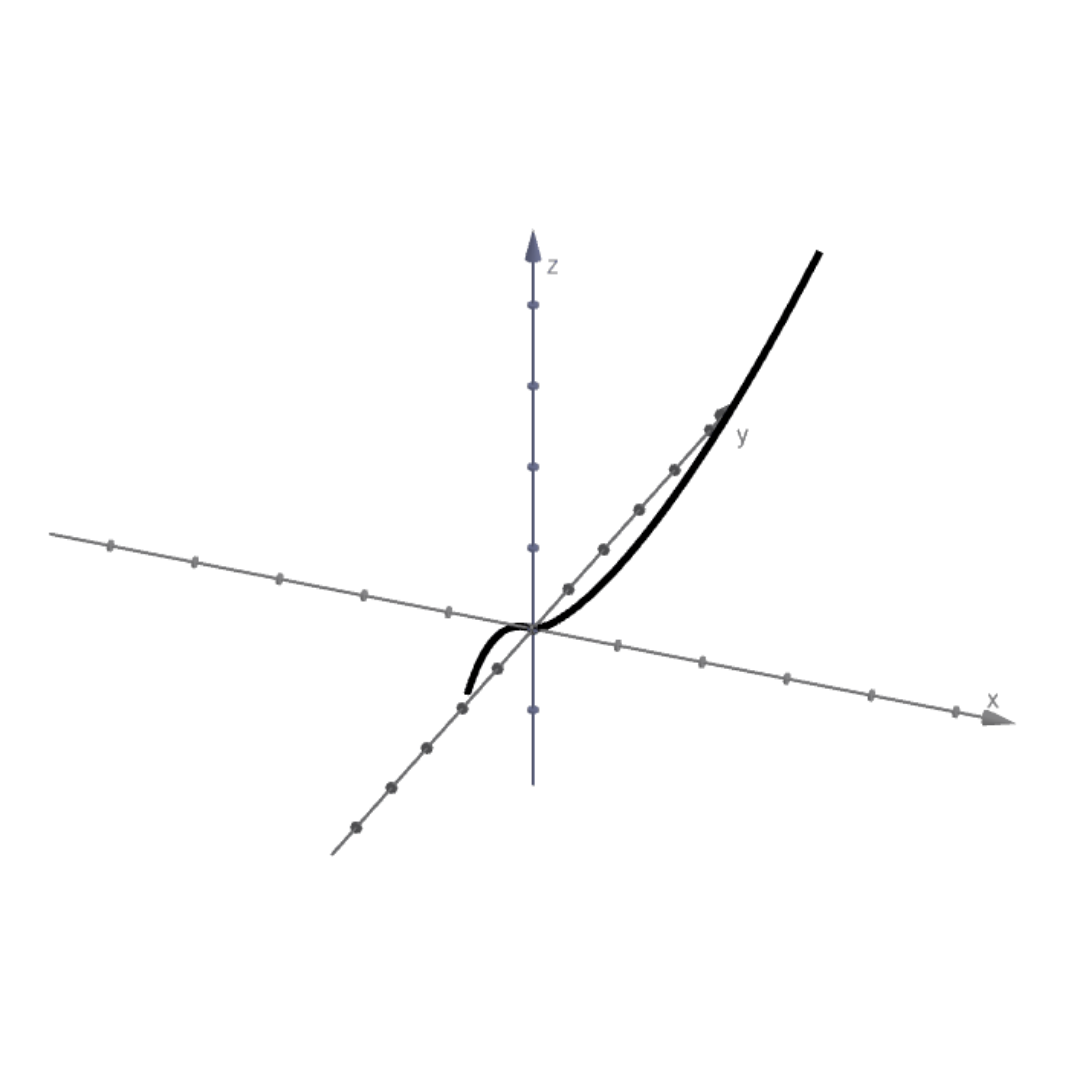
\includegraphics[width=0.3\linewidth]{Imagenes/Curva monomial}
				\caption{Curva monomial $Z(y^2-xz,yz-x^3,z^2-x^2y)$.}
				\label{fig:curva-monomial}
			\end{figure}
		\end{center}
   	\end{example}
    
    \begin{corollary}\label{analiticoafin}
    	Sea $V\subset \cc^n$ una variedad afín no singular de dimensión $r$. Entonces $V$ es una variedad compleja de dimensíon $r$.
    \end{corollary}
    \begin{proof}
    	Sea $p\in V$ un punto albitrario. Como $V$ es no singular de dimensión $r$, por el teorema \ref{teocarlos}, existe una vecindad $U_p\subset V$ de $p$ y polinomios 
    	\begin{equation*}
    		h_1,\dots,h_{n-r}\in\cc[z_1,\dots,z_n]
    	\end{equation*}
    	tales que
    	\begin{equation*}
    		V\cap U_p=\{q\in U_p:h_1(q)=\cdots=h_{n-r}(q)=0\},
    	\end{equation*}
    	y la matriz jacobiana $(\frac{\partial h_i}{\partial z_j}(p))$ tiene rango $n-r$.\\
    	De esto, $0\in \cc^{n-r}$ es un valor regular de la aplicación holomorfa $h=(h_1,\dots,h_{n-r}):U_p\subset\cc^n\to\cc^{n-r}$. Por el ejemplo \ref{interseccioncompleja}, $V\cap U_p$ es una variedad compleja de dimensión
    	\begin{equation*}
    		n-(n-r)=r.
    	\end{equation*}
    	Como $p$ fue cualquier punto, obtenemos una cubierta para $V$
    	\begin{equation*}
    		V=\bigcup_{p\in V}U_p.
    	\end{equation*} 
    	donde cada $U_p$ es una variedad compleja de dimensión $r$. Finalmente, aplicando el lema \ref{lemacubierta}, $V$ es una variedad compleja de dimensión $r$.
    \end{proof}
	
	Dado que toda variedad algebraica afín admite una estructura de variedad compleja, vale la pena preguntarnos si el recíproco es verdad. Es decir, toda variedad compleja se puede realizarse como una variedad algebraica afín. La respuesta a esta cuestión es negativa, pues en primer lugar, las variedades algebraicas afines son conjuntos cerrados de $\cc^n$. De hecho, incluso entre las variedades complejas cerradas en $\cc^n$ existen ejemplos no algebraicas. Esto significa que existen muchas más variedades complejas que variedades algebraicas, por lo que motiva el problema de determinar bajo qué condiciones una variedad compleja admite una realización algebraica.
	
	\begin{example}[Superficie de Riemann no algebraica]\label{graficadelseno}
		Sea
		\begin{equation*}
			X=\{(z,w)\in\mathbb \cc^2:\ w=\sin z\}
		\end{equation*}
		la gráfica de $\sin z$. Entonces $X$ es una superficie de Riemann (de hecho biholomorfa a $\cc$ mediante la proyección $\pi(z,\sin z)=z$) y no es compacta. Supongamos que existe un polinomio no cero $P(z,w)\in\cc[z,w]$ tal que
		\begin{equation*}
			P(z,\sin z)= 0\qquad\text{para todo }z\in\cc.
		\end{equation*}
		Escribamos
		\begin{equation*}
			P(z,w)=\sum_{j=0}^m a_j(z)w^j,\qquad a_j(z)\in\mathbb \cc[z].
		\end{equation*}
		Al evaluar en $w=0$ obtenemos el polinomio $a_0(z)=P(z,0) $. Como $P(z,\sin z)=0$, entonces para todo $z$ tal que $\sin z=0$ (es decir $z=n\pi,\ n\in\mathbb{Z}$) se cumple que $P(z,0)=0$. Así $a_0(z)$ tiene infinitos ceros y por ser un polinomio en $\cc[z]$ debe ser idénticamente cero.
		
		Con lo cual, $w$ divide a $P(z,w)$ en $\cc[z,w]$, es decir existe $P_1\in\cc[z,w] $ tal que
		\begin{equation*}
			P(z,w)=wP_1(z,w)
		\end{equation*}
		Con esto tenemos que
		\begin{equation*}
			0=P(z,\sin z)=\sin zP_1(z,\sin z),
		\end{equation*}
		y como $\sin z$ no es la función cero, entonces $ P_1(z,\sin z)=0$. Usando el mismo razonamiento, obtenemos que $P$ es divisible por $w^k$ para todo $k\geq 1$. Esto sólo es posible si $P$ es el polinomio cero, contradiciendo la hipótesis de que $P\neq0$. Por tanto, $X$ no es algebraica. 
		\begin{figure}[H]
			\centering
			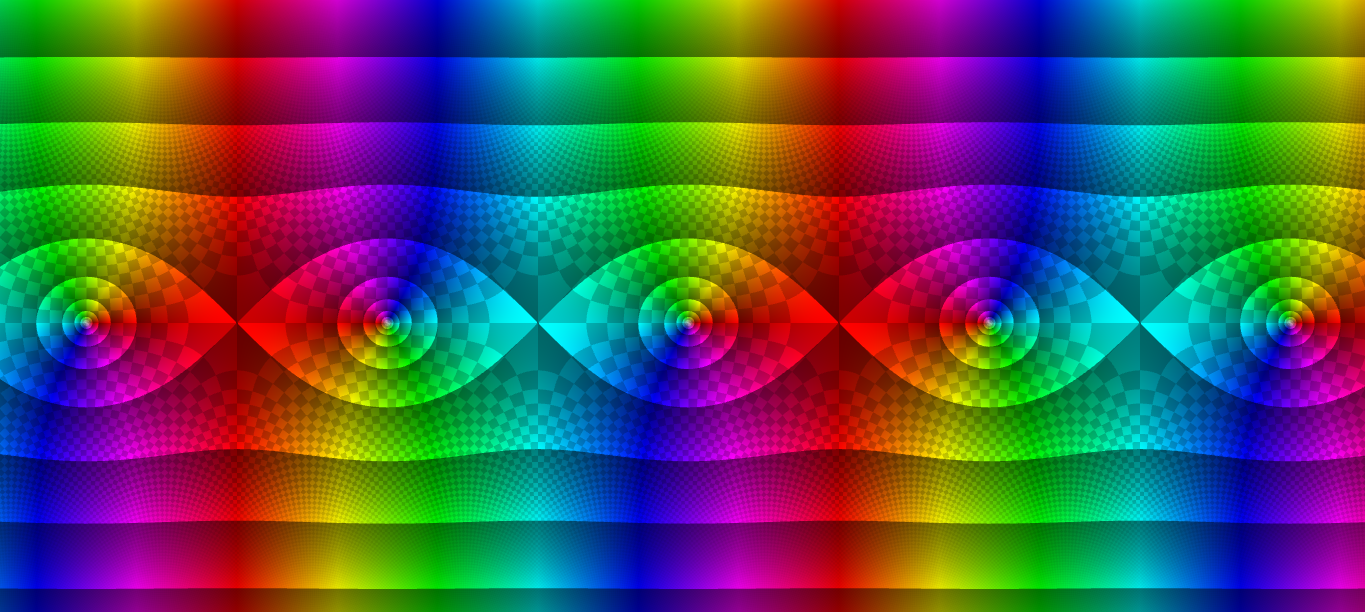
\includegraphics[width=0.5\linewidth]{Imagenes/Grafica del seno}
			\caption{Gráfica de la función seno}
%			\caption{La función seno tiene una cantidad infinita de ceros la recta $w=0$. Por lo tanto, si la gráfica del seno fuera algebraica, al intersectar con la recta $w=0$ debería ser algebraica, lo cual no es posible.}
			\label{fig:grafica-del-seno}
		\end{figure}
	\end{example}
    
  	Como ya mencionamos en la primera sección, la hipótesis de compacidad será bastante importante para buscar la algebrización y este último ejemplo no cumple con ser compacta. De esta manera, necesitamos también estudiar las variedades algebraicas que siempre son compactas.
  	
    Recordemos que $V\subset\pp^n$ es una variedad algebraica proyectiva (en general le llamaremos \textbf{variedad algebraica}) si es el conjunto de ceros de una cantidad finita de polinomios homogeneos, irreducible en la topología de Zariski. 
    
    \begin{definition}
%    	Sea $V\subset\pp^n$ una variedad algebraica y consideremos $V=\bigcup_{i=0}^n V_i$ la cubierta estandar afín. Definimos la \textbf{dimensión} de $V$ como el máximo de las dimensiones de las variedades afines $V_i\subset\cc^n$.
		Sea $V\subset\pp^n$ una variedad algebraica. Definimos la \textbf{dimensión} de $V$ como la dimensión de cualquiera de sus cartas fines no vacías.
    \end{definition}
    
    En particular, la dimensión es una propiedad local e intrinseca de la variedad  algebraica, sin importar el espacio ambierte donde se encuentre.
    
        \begin{remark}\label{dimcubierta}
    	Denotemos por $\cc(V)$ al campo de funciones racionales de la variedad algebraica (afín o proyectiva) $V$. De geometría algebraica (por ejemplo véase \parencite[Cap. 1 Sec. 3]{Harts}) sabemos que si $V$ es afín, entonces
    	\begin{equation*}
    		\trdeg_\cc \cc(V)=\dim V.
    	\end{equation*}
    	Además, si $V\subset \pp^n$ es una variedad algebraica que no está totalmente contenida en $Z(z_i)$, entonces 
    	\begin{equation*}
    		\cc(V)\cong \cc(V_i),\qquad \text{con }V_i\text{ como variedad afín}.
    	\end{equation*}
    	De esta manera, si $V\subset\pp^n$ es una variedad algebraica, entonces para cada $i=0,1,\dots, n$ 
    	\begin{equation*}
    		\cc(V)\cong \cc(V_i)
    	\end{equation*}
    	si $V$ no está totalmente contenida en $Z(z_i)$. Asi,
    	\begin{equation*}
    		\trdeg_\cc\cc(V)=\trdeg_\cc\cc(V_i)=\dim V_i.
    	\end{equation*}
    	Por lo tanto, la dimensión de todas las variedades afines $V_i$ es igual a la dimensión de la variedad $V$.
    \end{remark}
    
    \begin{definition}
    	Sea $V\subset\pp^n$ una variedad algebraica de dimensión $d$ y tomemos su cubierta afín
    	\begin{equation*}
    		V=\bigcup_{i=0}^n V_i
    	\end{equation*}
    	Decimos que la variedad $V$ es \textbf{no singular} si todos sus puntos son no singulares en todas las variedades afines. Es decir, las variedades afines $V_i$ son no singulares.
    \end{definition}
    
    Por definición, si $V\subset\pp^n$ es no singular, entonces $V$ está cubierta por $n+1$ variedades complejas (especificamente, está cubierto por abiertos en $V$ homeomorfos a una variedad compleja). Aprovecharemos esto para probar que $V$ también es una variedad compleja, pero determinemos antes las propiedades topológicas básicas de las variedades algebraicas.
    
    \begin{lemma}\label{topovariedades}
    	Toda variedad algebraica proyectiva es Hausdorff, segundo numerable y compacto (respecto a la topología compleja).
    \end{lemma}
    
    \begin{proof}
    	Sea $X\subset \pp^n$ una variedad algebraica proyectiva. Notemos que $X$ como subespacio de $\pp^n$ es Hausdorff y segundo numerable. Solo es necesario demostrar que es compacto. Consideremos $X_i=X\cap U_i$ la cubierta afín de $X$. Lo que haremos es demostrar que cada $X_i$ es cerrado. Así, $X$ será cerrado por ser unión finita de cerrados y como $\pp^n$ es compacto, entonces $X$ es compacto.\\
    	Como $X$ es variedad algebraica proyectiva, existen $F_k\in\cc[x_0,x_1,\dots,x_n]$ polinomios homogéneos tal que
    	\begin{equation*}
    		X=Z(F_1,F_2,\dots, F_k)        
    	\end{equation*}
    	Haremos la prueba para $i=0$, pero es análogo para todo $i=1,\dots, n$.
    	Notemos que
    	\begin{align*}
    		\phi_0(X_0)=Z(f_1,f_2,\dots, f_n)
    	\end{align*}
    	donde 
    	\begin{equation*}
    		f_j(x_1,\dots,x_n)=F_j\left(1,x_1,\dots,x_n\right)
    	\end{equation*}
    	para cada $j=1,2\dots,k$. Esto porque
    	\begin{align*}
    		\phi_0(X_i)&=\{\phi([1:x_1:\dots:x_n]):[1:x_1.\dots:x_n]\in X_i\}\\
    		&=\{(x_1,x_2,\dots,x_n):[1:x_1:\dots:x_n]\in X_i\}\\
    		&=\{(x_1,x_2,\dots,x_n):F_j[1:x_1:\dots:x_n]=0, \text{ para toda } j=1,2\dots k\}\\
    		&=\{(x_1,x_2,\dots,x_n):f_j(x_1,\dots,x_n)=0, \text{ para toda } j=1,2\dots k\}\\
    		&=Z(f_1,f_2,\dots,f_j)\subset \cc^n
    	\end{align*}
    	Así
    	\begin{equation*}
    		\phi_0(X_0)=Z(f_1,f_2,\dots,f_j)=\bigcap_{k=1}^jZ(f_k)=\bigcap_{k=1}^jf_k^{-1}(0)
    	\end{equation*}
    	Por lo tanto, $\phi_0(X_0)$ es cerrado por ser intersección de cerrados y como $\phi$ es un homeomorfismo, entonces $X_0$ es cerrado.
    \end{proof}
    
    La conexidad de las variedades algebraicas es un hecho para nada trivial, pero es una propiedad muy importante que necesitamos considerar. Una prueba de esta propiedad se puede consultar en \parencite[Cap. 4 Sec. 4.2]{carlosga} o en \parencite[Cap. VII Sec. 2]{shafarevich2016basic}. Más aún, también podemos verlo como un caso particular del teorema \ref{irreducibleconexo}. Por lo tanto, podemos concluir que:
    
    \begin{theorem}\label{varalg}
		Sea $V\subset\pp^n$ una variedad algebraica no singular de dimensión $r$. Entonces $V$ es una variedad compleja conexa compacta de dimensión $r$.    	
    \end{theorem}
   	\begin{proof}
   		Sea $V\subset\pp^n$ una variedad algebraica no singular de dimensión $r$ y consideremos su cubierta estándar 
   		\begin{equation*}
   			V=\bigcup_{i=0}^n V_i.
   		\end{equation*}
   		Supongamos que $V\not\subset Z(z_i)$ para todo $i=0,1,\dots,n$. Por la observación \ref{dimcubierta}, las variedades afines $V_i$ dimensión $r$. Luego, por definición de no singular, las $V_i$ son no singulares. De esta manera, por el corolario \ref{analiticoafin}, las variedades afines $V_i$ tienen estructura de variedad compleja de dimensión $r$.\\
   		Por el lema \ref{lemacubierta}, como $V$ está cubierto por las variedades complejas $V_i$, concluimos que $V$ tiene estructura de variedad compleja de dimensión $r$.\\
   		Ahora, si $V$ está totalmente contenida en algún $Z(z_i)$, digamos $i=0$, entonces $V_i=\emptyset$. Por lo que
   		\begin{equation*}
   			V=\bigcup_{i=0}^n V_i=\bigcup_{i=1}^n V_i
   		\end{equation*}
   		y la demostración sigue siendo válida.
   		
   		Por el lema \ref{topovariedades}, $V$ es compacta. Además, la conexidad de $V$ se sigue de la irreducibilidad de las variedades algebraicas proyectivas (véase la discusión previa al teorema). Por lo tanto, $V$ es una variedad compleja conexa y compacta de dimensión r.
   	\end{proof}

 
